\documentclass[12pt]{article}
 \usepackage[margin=1in]{geometry} 
\author{Joshua Stephenson-Losey,
Keefer Sands,
Taylor Koth}
\usepackage{amsmath,amsthm,amssymb,amsfonts}
\usepackage{centernot}
\usepackage[table]{xcolor}
\usepackage{algpseudocode}
\usepackage{algorithm}
\usepackage{graphicx}
\floatname{algorithm}{}
 
\newcommand{\N}{\mathbb{N}}
\newcommand{\Z}{\mathbb{Z}}
\renewcommand*{\proofname}{Solution}


\newenvironment{problem}[2][Problem]
{\begin{trivlist}
\item[\hskip \labelsep {\bfseries #1}\hskip \labelsep {\bfseries #2.}]}{\end{trivlist}}


\makeatletter
\renewcommand{\fnum@algorithm}{\fname@algorithm}
\makeatother

\begin{document}

 
\title{CSCI 432\\Homework 5}
\date{}
\maketitle

Assigned 10/31/2018, due by end of class (4:00 pm) on 11/26/2018. Marked questions (*) are graded for correctness. The remaining will be graded for effort. Please see the course website for details about expected effort.

You must follow the collaboration policy detailed on the course website. Please type solutions in an appropriate editor (\LaTeX, Word) so that I can review equations and proofs efficiently. 

\begin{problem}{1*}
Provide a graph that the vertex cover approximation algorithm always will find a suboptimal solution for.
\end{problem}


\begin{problem}{2*}
The Clique problem is: Given a graph, find the largest complete subgraph (i.e. largest subgraph where each pair of vertices share an edge). Given a graph $G$, the complement graph is the graph containing exactly the edges not in $G$. In other words, if $e=(u,v)$ is an edge in $G$, it is not in the complement graph. If $(x,y)$ is not an edge in $G$, then it is in the complement graph. An example of a graph and its complement is shown below. Show that a Clique of size $k$ in some graph $G$ is a Vertex Cover of size $|V|-k$ in the complement graph.

\begin{figure}[H]
\centering
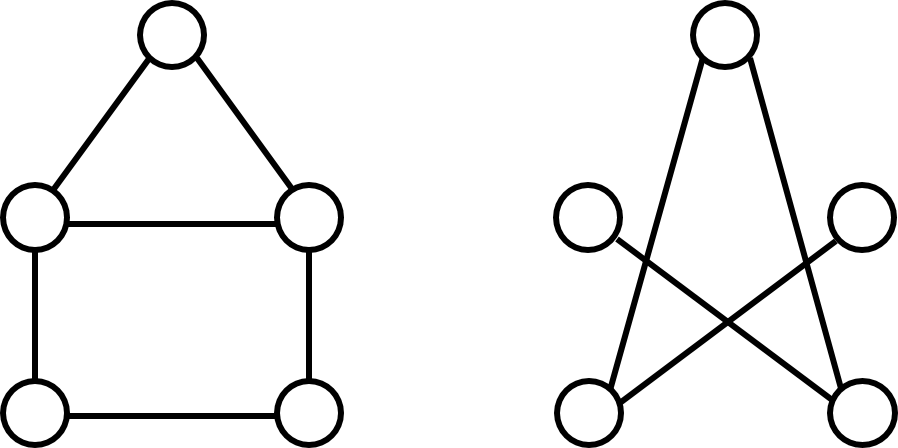
\includegraphics[scale=.5]{Homework5_comp.png}
\end{figure}
\end{problem}


\begin{problem}{3}
Since the complement of an optimal Vertex Cover gives a Clique of maximum size, does the $2$-approximation algorithm for Vertex Cover provide a constant ratio approximation algorithm for the Clique problem?
\end{problem}


\begin{problem}{4*}
The Minimum Dominating Set problem is: Given a graph, find the smallest subset of the vertices such that each remaining vertex has a neighbor in the selected subset. Find an approximation algorithm for the Minimum Dominating Set problem (hint: Draw it out and see if it seems similar to a problem we studied in class).
\end{problem}


\begin{problem}{5}
Show up and participate in the workshop session on 11/9.
\end{problem}

\end{document}